% ============================================================
%  BEAMER — CLASE 2: NÚMEROS ENTEROS Y SUS OPERACIONES
%  Curso Introductorio de Matemáticas · 1er Año
%  Autor: Ing. Gabriel Astudillo
%  Compilar: latexmk -xelatex beamer2_numeros_enteros.tex
%  Cubre: suma/resta, multiplicación/división y operaciones
%         combinadas en Z (jerarquía y signos de agrupación).
% ============================================================
\documentclass[aspectratio=169]{beamer}
\usepackage{mathwizards-beamer}
\mwbeamer{Clase 2}{Los Números Enteros y sus Operaciones}{Curso 1er Año}

% ── Comandos propios de esta clase ───────────────────────────
\newcommand{\Z}{\mathbb{Z}}

\begin{document}

\begin{frame}[plain]
  \titlepage
\end{frame}

% ════════════════════════════════════════════════════════════
\section{El Conjunto de los Números Enteros}
% ════════════════════════════════════════════════════════════

\begin{frame}{El Conjunto $\Z$}
  \begin{block}{Definición}
    \[
      \Z = \{\dots, -3, -2, -1, 0, 1, 2, 3, \dots\}
    \]
    \begin{itemize}
      \item Los \textbf{positivos} ($1, 2, 3, \dots$) están a la derecha del cero.
      \item Los \textbf{negativos} ($-1, -2, -3, \dots$) están a la izquierda del cero.
      \item El \textbf{cero} no es positivo ni negativo: es el punto de partida.
    \end{itemize}
  \end{block}
  \vspace{6pt}
  \begin{center}
    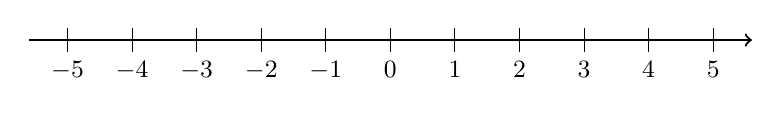
\begin{tikzpicture}[x=0.82cm]
      \draw[->, thick] (-5.6,0) -- (5.6,0);
      \foreach \x in {-5,-4,...,5} {
        \draw (\x,0.15) -- (\x,-0.15) node[below] {\small $\x$};
      }
    \end{tikzpicture}
  \end{center}
  \vspace{2pt}
  \begin{mwextra}[Interpretación]
    Caminar a la \textbf{derecha} es \textbf{sumar}; caminar a la \textbf{izquierda} es \textbf{restar}.
  \end{mwextra}
\end{frame}

\begin{frame}{Valor Absoluto}
  \begin{block}{Definición}
    El \textbf{valor absoluto} de $a \in \Z$, escrito $|a|$, es la \emph{distancia} de $a$ hasta el cero en la recta numérica. Siempre es positiva o cero.
    \[
      |5| = 5 \qquad |-5| = 5 \qquad |0| = 0
    \]
  \end{block}
  \vspace{6pt}
  \begin{mwextra}[Idea clave]
    $-5$ y $5$ están a la misma distancia del cero, por eso $|-5| = |5| = 5$.
  \end{mwextra}
\end{frame}

% ════════════════════════════════════════════════════════════
\section{Suma y Resta en $\Z$}
% ════════════════════════════════════════════════════════════

\begin{frame}{Suma y Resta: Regla de los Signos}
  \begin{block}{Dos casos}
    \begin{itemize}
      \item \textbf{Igual signo:} se suman los valores y se conserva el signo.
            \[
              -4 + (-3) = -7 \qquad\qquad 5 + 8 = 13
            \]
      \item \textbf{Signos diferentes:} se restan los valores absolutos y se coloca el signo del número con mayor valor absoluto.
            \[
              -7 + 4 = -3 \qquad\qquad 7 + (-4) = 3
            \]
    \end{itemize}
  \end{block}
  \vspace{4pt}
  \begin{exampleblock}{Restar es sumar el opuesto}
    \[
      a - b = a + (-b) \qquad\Longrightarrow\qquad 5 - 9 = 5 + (-9) = -4
    \]
  \end{exampleblock}
\end{frame}

\begin{frame}{Los Signos Dobles}
  \begin{alertblock}{Cuatro combinaciones}
    \[
      +\,(+)=+ \qquad +\,(-)=- \qquad -\,(+)=- \qquad -\,(-)=+
    \]
    Signos iguales dan $+$; signos distintos dan $-$.
  \end{alertblock}
  \vspace{6pt}
  \begin{block}{Ejemplos}
    \[
      8 - (-3) = 8 + 3 = 11 \qquad\qquad -5 + (-2) = -5 - 2 = -7
    \]
  \end{block}
\end{frame}

\begin{frame}{Ejemplo Resuelto}
  \begin{block}{Situación}
    En la mañana la temperatura era de $-4\,^{\circ}$C y subió $10\,^{\circ}$C. \textquestiondown Cuál es la nueva temperatura?
  \end{block}
  \vspace{6pt}
  \begin{mwextra}[Solución]
    \[
      -4 + 10 = 6
    \]
    La nueva temperatura es $6\,^{\circ}$C.
  \end{mwextra}
\end{frame}

% ════════════════════════════════════════════════════════════
\section{Multiplicación y División en $\Z$}
% ════════════════════════════════════════════════════════════

\begin{frame}{Multiplicación y División: Regla de los Signos}
  \begin{columns}[T]
    \column{0.42\textwidth}
    \begin{block}{Tabla de signos}
      \begin{center}
        \begin{tabular}{cc|c}
          \toprule
          \textbf{Sig.} & \textbf{Sig.} & \textbf{Result.} \\
          \midrule
          $+$ & $+$ & $+$ \\
          $+$ & $-$ & $-$ \\
          $-$ & $+$ & $-$ \\
          $-$ & $-$ & $+$ \\
          \bottomrule
        \end{tabular}
      \end{center}
    \end{block}
    \column{0.54\textwidth}
    \begin{mwextra}[Truco: amigo / enemigo]
      \begin{itemize}
        \item Amigo de mi amigo $\rightarrow$ \textbf{amigo} \quad ($+\times +=+$)
        \item Amigo de mi enemigo $\rightarrow$ \textbf{enemigo} \quad ($+\times -= -$)
        \item Enemigo de mi amigo $\rightarrow$ \textbf{enemigo} \quad ($-\times +=-$)
        \item Enemigo de mi enemigo $\rightarrow$ \textbf{amigo} \quad ($-\times -=+$)
      \end{itemize}
    \end{mwextra}
  \end{columns}
\end{frame}

\begin{frame}{Casos Especiales}
  \begin{alertblock}{Atención}
    \begin{itemize}
      \item Cero por cualquier número da cero: \quad $0 \times (-7) = 0$.
      \item Cero dividido entre un número no nulo da cero: \quad $0 \div (-4) = 0$.
      \item \textbf{No se puede dividir entre cero.} \quad ($a \div 0$ \quad ¡prohibido!)
    \end{itemize}
  \end{alertblock}
  \vspace{6pt}
  \begin{block}{Ejemplos}
    \[
      (-4) \times (-3) = 12 \qquad\qquad (-20) \div (-4) = 5
    \]
  \end{block}
\end{frame}

\begin{frame}{Ejemplo Resuelto}
  \begin{block}{Buceador}
    Un buceador desciende $3$ metros cada minuto. \textquestiondown A qué profundidad estará después de $4$ minutos?
  \end{block}
  \vspace{6pt}
  \begin{mwextra}[Solución]
    ``Bajar'' es negativo: \quad $4 \times (-3) = -12$.\\[4pt]
    Estará a $-12$ m (es decir, $12$ m bajo el agua).
  \end{mwextra}
\end{frame}

% ════════════════════════════════════════════════════════════
\section{Operaciones Combinadas}
% ════════════════════════════════════════════════════════════

\begin{frame}{Jerarquía de las Operaciones}
  \begin{mwpasos}[Orden para resolver]
    \begin{enumerate}
      \item Primero \textbf{multiplicaciones y divisiones}, de izquierda a derecha.
      \item Luego \textbf{sumas y restas}, de izquierda a derecha.
    \end{enumerate}
  \end{mwpasos}
  \vspace{6pt}
  \begin{alertblock}{\textquestiondown Multiplicación o división primero?}
    Si aparecen consecutivas sin signos de agrupación, se resuelven \emph{de izquierda a derecha}:
    \[
      4 \cdot (-3) : (-2) : (-6) = (-12) : (-2) : (-6) = 6 : (-6) = -1
    \]
  \end{alertblock}
\end{frame}

\begin{frame}{Signos de Agrupación}
  \begin{mwpasos}[De adentro hacia afuera]
    \begin{enumerate}
      \item Paréntesis \quad $(\;\;)$
      \item Corchetes \quad $[\;\;]$
      \item Llaves \quad $\{\;\;\}$
    \end{enumerate}
    Dentro de cada nivel se respeta la jerarquía estándar (multiplicación/división antes que suma/resta).
  \end{mwpasos}
  \vspace{6pt}
  \begin{exampleblock}{Ejemplo}
    \[
      [6 - (-1) - (-13)] : (-5) = 20 : (-5) = -4
    \]
  \end{exampleblock}
\end{frame}

\begin{frame}{Ejemplo Multinivel}
  \begin{block}{Resuelve}
    \[
      18 : [\,6 - 3 \cdot (-4 : 2 + 1)\,] - 3
    \]
  \end{block}
  \vspace{6pt}
  \begin{mwpasos}[Paso a paso]
    \begin{itemize}
      \item Paréntesis: \; $-4 : 2 + 1 = -2 + 1 = -1$.
      \item Corchete: \; $6 - 3 \cdot (-1) = 6 + 3 = 9$.
      \item División: \; $18 : 9 = 2$.
      \item Resta: \; $2 - 3 = -1$.
    \end{itemize}
  \end{mwpasos}
\end{frame}

% ════════════════════════════════════════════════════════════
\section{Ejercicios de Clase}
% ════════════════════════════════════════════════════════════

\begin{frame}{Ejercicio 1}
  \begin{mwejercicio}[Operaciones combinadas \quad \facil]
    $6 - 4 \cdot (-3) + 5$
  \end{mwejercicio}
\end{frame}

\begin{frame}{Ejercicio 2}
  \begin{mwejercicio}[Operaciones combinadas \quad \facil]
    $(-15) : 3 + (-8) \cdot (-2)$
  \end{mwejercicio}
\end{frame}

\begin{frame}{Ejercicio 3}
  \begin{mwejercicio}[Operaciones combinadas \quad \facil]
    $(-3 + 6 + 18) : (-3)$
  \end{mwejercicio}
\end{frame}

\begin{frame}{Ejercicio 4}
  \begin{mwejercicio}[Operaciones combinadas \quad \medio]
    $[2 - (-5) - 3] \cdot (-2)$
  \end{mwejercicio}
\end{frame}

\begin{frame}{Ejercicio 5}
  \begin{mwejercicio}[Operaciones combinadas \quad \medio]
    $12 : (-4) \cdot 3 - (-8) + 5$
  \end{mwejercicio}
\end{frame}

\begin{frame}{Ejercicio 6}
  \begin{mwejercicio}[Operaciones combinadas \quad \medio]
    $[6 - (-1) - (-13)] : (-5)$
  \end{mwejercicio}
\end{frame}

\begin{frame}{Ejercicio 7}
  \begin{mwejercicio}[Operaciones combinadas \quad \medio]
    $-4 + 6 \cdot (-2 + 5) : (-9) + 2 \cdot 3$
  \end{mwejercicio}
\end{frame}

\begin{frame}{Ejercicio 8}
  \begin{mwejercicio}[Operaciones combinadas \quad \dificil]
    $18 : [\,6 - 3 \cdot (-4 : 2 + 1)\,] - 3$
  \end{mwejercicio}
\end{frame}

\begin{frame}{Ejercicio 9}
  \begin{mwejercicio}[Operaciones combinadas \quad \dificil]
    $\{\,[-4 + 6 \cdot (-2 + 5)] : (-7) + 2\,\} \cdot 3$
  \end{mwejercicio}
\end{frame}

\begin{frame}{Ejercicio 10}
  \begin{mwejercicio}[Operaciones combinadas \quad \dificil]
    $-2 \cdot \{\,-5 + 3 \cdot [-4 - (-12 : 3 + 1)]\,\} - (-10)$
  \end{mwejercicio}
\end{frame}

\begin{frame}{Cierre}
  \begin{exampleblock}{¡Excelente trabajo!}
    Ya dominas los signos, la jerarquía de las operaciones y los signos de agrupación en $\Z$.\\[6pt]
    En la próxima clase conoceremos la \textbf{potenciación}: multiplicar un número por sí mismo varias veces.
  \end{exampleblock}
\end{frame}

\end{document}
